\documentclass[conference]{IEEEtran}
\IEEEoverridecommandlockouts
\usepackage{cite}
\usepackage{amsmath,amssymb}
\usepackage{graphicx}
\usepackage{booktabs}
\usepackage{multirow}
\usepackage{xcolor}
\usepackage{tikz}
\usetikzlibrary{positioning,arrows.meta}
\usepackage[hidelinks]{hyperref}
\usepackage{url}

\newcommand{\best}[1]{\textbf{#1}}

\begin{document}

\title{CNNs, Vision Transformers and a CNN--Transformer Hybrid for Gastrointestinal Endoscopy Classification: Accuracy, Cost, Interpretability and Shortcut Learning on Kvasir v2}

\author{\IEEEauthorblockN{Jon\'as Ariel Acu\~na G\'omez}
\IEEEauthorblockA{\textit{Master's Program in Artificial Intelligence} \\
\textit{Universidad Panamericana}\\
Mexico City, Mexico \\
jonasacuna28@gmail.com}}

\maketitle

\begin{abstract}
We compare four deep-learning architectures for the eight-class classification of gastrointestinal endoscopy images
(Kvasir v2, 8{,}000 images) under a single experimental protocol: a classic CNN (ResNet-50), an efficient CNN
(EfficientNet-B0), a pure Vision Transformer (ViT-S/16) and a CNN--Transformer hybrid built for this study
(ResNet-50 stages 1--3 followed by four Transformer layers), plus a soft-voting ensemble selected on the validation
set. Besides accuracy and macro-F1 with bootstrap confidence intervals and McNemar tests, we report parameters, MACs,
training time, GPU memory, latency and convergence, a one-factor-at-a-time hyperparameter study, Grad-CAM and attention
rollout maps, and a shortcut-learning test based on an acquisition artifact. All models exceed 0.90 macro-F1. ViT-S/16
is the best single model (0.936, 93.6\,\% accuracy) and is significantly better than the other three, but it was also
pretrained on ten times more data. Pretraining dominates every architectural choice: training from scratch costs 0.19
to 0.26 macro-F1, six to nine times the spread between the pretrained models, and explains why the hybrid, with 47\,\%
of its weights randomly initialized, is the weakest model. EfficientNet-B0 reaches 97\,\% of the best score with
1/12 of the compute. Most remaining errors confuse esophagitis with the normal Z-line, and every model partly relies
on a colonoscopy-only display box (0.014--0.034 macro-F1 lost when it is masked).
\end{abstract}

\begin{IEEEkeywords}
medical image classification, gastrointestinal endoscopy, Kvasir, convolutional neural networks, vision transformers, transfer learning, interpretability, shortcut learning
\end{IEEEkeywords}

\section{Introduction}
Endoscopy is the reference examination of the gastrointestinal (GI) tract, but its yield depends on the attention and
experience of the endoscopist: subtle lesions and early inflammation are missed, and the interpretation of findings
varies between observers. Computer-aided detection and classification systems can act as a second reader, and deep
learning has become the dominant approach since the release of public datasets such as Kvasir~\cite{pogorelov2017kvasir}
and HyperKvasir~\cite{borgli2020hyperkvasir}.

For a decade, convolutional neural networks (CNNs) such as ResNet~\cite{he2016resnet} and
EfficientNet~\cite{tan2019efficientnet} were the default choice. Vision Transformers (ViT)~\cite{dosovitskiy2021vit}
replace convolutions with global self-attention and lead natural-image benchmarks when enough pretraining data is
available, while hybrids combine a convolutional stem with Transformer layers~\cite{dosovitskiy2021vit,chen2021transunet,dai2021coatnet}.
Whether these advances carry over to small medical datasets is not obvious: Transformers lack the locality bias of
convolutions and depend heavily on pretraining~\cite{steiner2022augreg,matsoukas2021time}.

This work answers four questions on Kvasir v2 under a single, fully reproducible protocol: (i)~which family works best
on a small dataset (5{,}600 training images) and why; (ii)~what each model costs and how fast it converges; (iii)~where
the models look and whether they exploit shortcuts; and (iv)~how sensitive the conclusions are to the main
hyperparameters. Our contributions are:
\begin{itemize}
\item A compute-matched comparison of ResNet-50, EfficientNet-B0 and ViT-S/16, and a CNN--Transformer hybrid built for
this study, with significance tests and a complete cost profile (parameters, MACs, time, memory, latency, convergence).
\item A one-factor-at-a-time sensitivity study (learning rate, batch size, resolution, augmentation, pretraining),
including from-scratch training of a CNN and a Transformer.
\item The identification and quantification of a shortcut in Kvasir v2: a display box present only in colonoscopies,
on which every model partly relies.
\end{itemize}

\section{Related Work}
\textbf{GI endoscopy datasets and benchmarks.} Kvasir~\cite{pogorelov2017kvasir} introduced eight classes of anatomical
landmarks, pathological findings and endoscopic procedures annotated by endoscopists; its second version, used here,
has 1{,}000 images per class. The MediaEval Medico tasks~\cite{pogorelov2018medico} built on it and established
transfer learning from ImageNet as the dominant approach. HyperKvasir~\cite{borgli2020hyperkvasir} extended it to 23
classes and more than 100k unlabeled frames, and Kvasir-SEG~\cite{jha2020kvasirseg} added polyp segmentation masks.
Thambawita \emph{et al.}~\cite{thambawita2020extensive} showed that models trained on one GI dataset generalize poorly to
another, which motivates the analysis of dataset-specific cues in this work.

\textbf{CNNs and Transformers in medical imaging.} CNNs pretrained on ImageNet have been the standard in medical image
analysis~\cite{litjens2017survey}, although Raghu \emph{et al.}~\cite{raghu2019transfusion} showed that the benefit of
transfer learning shrinks for large medical datasets. ViT~\cite{dosovitskiy2021vit} needs large-scale pretraining;
DeiT~\cite{touvron2021deit} and AugReg~\cite{steiner2022augreg} reduced this need with stronger training recipes, and
Swin~\cite{liu2021swin} reintroduced locality through shifted windows. In medical imaging, Matsoukas
\emph{et al.}~\cite{matsoukas2021time} found that ImageNet-pretrained ViTs match CNNs while CNNs win when both are trained
from scratch, and Shamshad \emph{et al.}~\cite{shamshad2023survey} review the rapid adoption of Transformers.
Hybrid designs, such as the ResNet--ViT hybrid of the original ViT paper~\cite{dosovitskiy2021vit},
TransUNet~\cite{chen2021transunet} and CoAtNet~\cite{dai2021coatnet}, combine convolutional feature extraction with
global attention.

\textbf{Interpretability and shortcuts.} Grad-CAM~\cite{selvaraju2017gradcam} and attention
rollout~\cite{abnar2020rollout} are the usual tools to inspect where CNNs and Transformers look. Shortcut
learning~\cite{geirhos2020shortcut}, where a model exploits a spurious cue correlated with the label, has been documented
in medical imaging, e.g.\ for COVID-19 radiographs~\cite{degrave2021covid}.

\section{Methodology}
\subsection{Dataset and split}
Kvasir v2 contains 8{,}000 JPEG images (720$\times$576 to 1920$\times$1072 pixels) in eight balanced classes:
dyed-lifted polyps, dyed resection margins, esophagitis, normal cecum, normal pylorus, normal Z-line, polyps and
ulcerative colitis (Fig.~\ref{fig:examples}). We use a stratified 70/15/15 split (5{,}600/1{,}200/1{,}200 images,
seed 42). The validation set drives early stopping and the ensemble selection; the test set is used once.
Because the classes are balanced, no re-weighting or re-sampling is needed.

\begin{figure}[t]
\centering
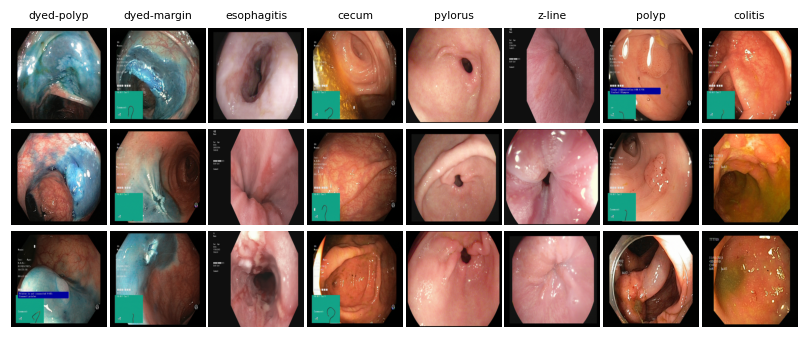
\includegraphics[width=\columnwidth]{figures/examples.png}
\caption{Kvasir v2 examples (three per class). The teal box in the lower-left corner of several colon images is the
ScopeGuide display (Section~\ref{sec:shortcut}).}
\label{fig:examples}
\end{figure}

\subsection{Preprocessing and augmentation}
Images are resized once to 256$\times$256 and cached. Training uses a random 224$\times$224 crop, horizontal and
vertical flips, rotations of $\pm$15$^\circ$ and brightness/contrast changes of $\pm$10\,\%; validation and test use a
center crop. Flips and rotations are valid because an endoscope has no canonical orientation. Hue and saturation are
\emph{not} altered because color is diagnostic: the indigo-carmine dye separates dyed from non-dyed polyps, and redness
indicates inflammation. Each model is normalized with the statistics of its own pretraining (ImageNet mean/std for the
CNNs, 0.5/0.5 for the AugReg ViT). Augmentation runs on the GPU with a single affine resampling per batch.

\subsection{Models}
\textbf{ResNet-50}~\cite{he2016resnet} (23.5\,M parameters, 4.1 GMACs). ResNet-18/34 have less capacity, and
ResNet-101/152 cost two to three times more compute for one to two ImageNet points, a gain unlikely to transfer to
5{,}600 images. ResNet-50 is the usual CNN baseline in the Kvasir literature. Weights: torchvision's improved recipe.

\textbf{EfficientNet-B0}~\cite{tan2019efficientnet} (4.0\,M, 0.38 GMACs). EfficientNet scales depth, width and input
resolution jointly; B0 is the only variant designed for 224\,px, which keeps the input identical for all models.

\textbf{ViT-S/16}~\cite{dosovitskiy2021vit} (21.7\,M, 4.6 GMACs), pretrained on ImageNet-21k with the AugReg
recipe~\cite{steiner2022augreg}. Its compute matches ResNet-50, so their comparison isolates convolution versus
self-attention rather than budget. ViT-Ti is too small, ViT-B is four times more expensive, and Swin-T's local windows
would blur the CNN--Transformer contrast.

\textbf{Hybrid ResNet-50 + Transformer} (16.1\,M, 4.9 GMACs), built for this study (Fig.~\ref{fig:hybrid}). The
pretrained ResNet-50 stem and stages 1--3 produce a 14$\times$14$\times$1024 map that is projected to 384 channels,
flattened into 196 tokens, prepended with a class token and added to learned position embeddings, and processed by four
pre-norm Transformer layers (6 heads, MLP 1536, dropout 0.1). The design follows the ViT hybrid~\cite{dosovitskiy2021vit}
and the TransUNet encoder~\cite{chen2021transunet}: the CNN extracts local texture, attention relates distant regions.
Cutting after stage 3 keeps 196 tokens (stage 4 would leave 49) and makes the hybrid a controlled variant of ResNet-50
in which stage 4 and global pooling are replaced by attention. Its 7.6\,M new parameters (47\,\%) are randomly
initialized.

\begin{figure}[t]
\centering
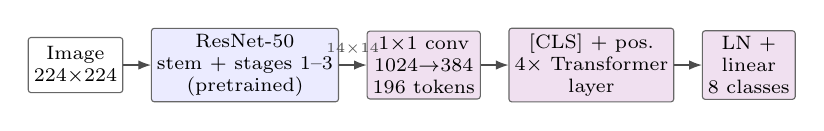
\begin{tikzpicture}[font=\scriptsize, node distance=3.5mm,
  box/.style={draw=black!60, rounded corners=1pt, align=center, minimum height=7mm, inner sep=2pt},
  pre/.style={box, fill=blue!8}, new/.style={box, fill=violet!12}, arr/.style={-{Latex[length=1.6mm]}, black!70}]
\node[box] (in) {Image\\224$\times$224};
\node[pre, right=of in] (cnn) {ResNet-50\\stem + stages 1--3\\(pretrained)};
\node[new, right=of cnn] (proj) {1$\times$1 conv\\1024$\rightarrow$384\\196 tokens};
\node[new, right=of proj] (tr) {[CLS] + pos.\\4$\times$ Transformer\\layer};
\node[new, right=of tr] (head) {LN +\\linear\\8 classes};
\draw[arr] (in) -- (cnn); \draw[arr] (cnn) -- node[above, font=\tiny]{14$\times$14} (proj); \draw[arr] (proj) -- (tr); \draw[arr] (tr) -- (head);
\end{tikzpicture}
\caption{The hybrid built in this work. Blue: pretrained weights (LR $10^{-4}$); violet: new layers trained from scratch (LR $10^{-3}$).}
\label{fig:hybrid}
\end{figure}

\subsection{Training protocol}
All models share the protocol of Table~\ref{tab:protocol}. The same seed fixes initialization, batch order and
augmentation. Training runs on one NVIDIA L4 GPU with bfloat16 mixed precision.

\begin{table}[t]
\caption{Shared training protocol and rationale}
\label{tab:protocol}
\centering
\footnotesize
\setlength{\tabcolsep}{3pt}
\begin{tabular}{@{}p{2.05cm}p{1.75cm}p{4.1cm}@{}}
\toprule
Setting & Value & Rationale \\
\midrule
Input & 224\,px & Native resolution of all pretrained weights \\
Optimizer & AdamW & Decoupled weight decay~\cite{loshchilov2019adamw}; standard for CNN and ViT fine-tuning \\
Learning rate & $10^{-4}$ & Fine-tuning; hybrid's new layers $10^{-3}$ \\
Schedule & 1-epoch warm-up + cosine & Protects pretrained weights from the random head's early gradients~\cite{goyal2017large,loshchilov2017sgdr} \\
Batch size & 32 & 175 updates per epoch; small-batch noise regularizes \\
Weight decay & 0.05 & Not applied to biases, norms, position embeddings \\
Label smoothing & 0.1 & Less over-confidence, better-calibrated probabilities~\cite{szegedy2016rethinking} \\
Epochs & $\le$20, patience 4 & Early stopping on validation macro-F1 \\
Grad.\ clipping & norm 1.0 & Guards against gradient spikes \\
\bottomrule
\end{tabular}
\end{table}

\subsection{Evaluation}
The primary metric is test macro-F1, the unweighted mean of the per-class F1 scores, which prevents a weak class from
hiding behind strong ones; we also report accuracy, per-class F1 and confusion matrices. 95\,\% confidence intervals are
obtained with 1{,}000 paired bootstrap resamples of the test set~\cite{efron1993bootstrap}, and pairs of models are
compared with the exact McNemar test~\cite{mcnemar1947,dietterich1998tests}. Cost is measured as parameters,
multiply-accumulate operations (MACs), training time, peak GPU memory, throughput (batch 64) and single-image latency.
Convergence is measured as the best epoch and the number of epochs to reach 95\,\% of the best validation macro-F1.
Success criteria fixed before training: every model $\ge$0.90 macro-F1; differences claimed only if $p<0.05$; the best
model loses $\le$0.02 macro-F1 when the shortcut is removed.

\textbf{Ensemble.} All 11 soft-voting combinations of two or more models are scored on the validation set; the best
(ties broken by size) is evaluated once on the test set.

\textbf{Sensitivity.} Starting from the EfficientNet-B0 configuration, each run changes one factor: learning rate
($10^{-5}$, $10^{-3}$), batch size (128, same LR), resolution (64\,px), no augmentation, and random initialization. One
extra run trains ViT-S/16 from scratch.

\textbf{Interpretability and shortcut test.} Grad-CAM~\cite{selvaraju2017gradcam} is computed on the last convolutional
map of each CNN (and of the hybrid's CNN part) and attention rollout~\cite{abnar2020rollout} on the Transformer layers.
The ScopeGuide box is located from the data (teal pixels: $G>100$, $G-R>60$, $G>B$), masked in the test images, and the
models are re-evaluated without retraining. We also compute the share of each explanation map that falls inside the
box, divided by the box's share of the image area (1 = uniform).

\section{Results}
\subsection{Overall performance}
Table~\ref{tab:main} summarizes the test results. All models meet the 0.90 criterion. ViT-S/16 is the best single
model (macro-F1 0.936) and is significantly better than ResNet-50 ($p=0.041$), EfficientNet-B0 ($p=0.002$) and the
hybrid ($p<0.001$). The three CNN-based models are not significantly different from each other ($p=0.07$--$0.54$).
The ensemble selected on validation, ViT-S/16 + Hybrid, has the highest point estimate (0.938), but its gain over
ViT-S/16 is not significant ($p=0.63$; 10 versus 7 discordant images). The full run took 44.7 minutes.

\begin{table*}[t]
\caption{Test results (1{,}200 images). Macro-F1 and accuracy with 95\,\% bootstrap CIs; McNemar $p$ against ViT-S/16.
Cost of the ensemble is the sum of its members. Latency: one image; throughput: batch of 64 (NVIDIA L4, bf16).}
\label{tab:main}
\centering
\footnotesize
\setlength{\tabcolsep}{4pt}
\resizebox{\textwidth}{!}{%
\begin{tabular}{@{}lcccccccccc@{}}
\toprule
Model & Macro-F1 [95\,\% CI] & Acc.\ (\%) & $p$ vs ViT & Params (M) & GMACs & Train (s) & Memory (MB) & Latency (ms) & Thr.\ (ms/img) & Best / run ep. \\
\midrule
Ensemble ViT-S + Hybrid & \best{0.938} [0.925, 0.952] & \best{93.83} & 0.63 & 37.8 & 9.47 & 353 & -- & 17.56 & 1.26 & -- \\
ViT-S/16 & 0.936 [0.923, 0.949] & 93.58 & -- & 21.7 & 4.60 & 190 & 1545 & \best{7.20} & 0.45 & 19 / 20 \\
ResNet-50 & 0.921 [0.906, 0.935] & 92.08 & 0.041 & 23.5 & 4.09 & 246 & 1909 & 8.86 & 0.74 & 12 / 16 \\
EfficientNet-B0 & 0.912 [0.897, 0.927] & 91.25 & 0.002 & \best{4.0} & \best{0.38} & 210 & \best{1492} & 11.35 & \best{0.39} & 15 / 19 \\
Hybrid R50 + Transformer & 0.906 [0.890, 0.923] & 90.67 & $<$0.001 & 16.1 & 4.87 & \best{162} & 2089 & 10.36 & 0.81 & 6 / 10 \\
\bottomrule
\end{tabular}}
\end{table*}

\subsection{Cost and convergence}
Fig.~\ref{fig:cost} relates performance and cost. EfficientNet-B0 reaches 97\,\% of the best macro-F1 with about one
fifth of ViT-S's parameters and one twelfth of its MACs, and has the best batched throughput. Yet, with a single image,
it is the slowest model (11.3\,ms versus 7.2\,ms for ViT-S/16): its many small depthwise layers are bound by memory
access and kernel launches rather than arithmetic, whereas ViT-S maps to a few large matrix products. All models are
far below the 33\,ms frame budget of a 30\,fps video.

All models reach 95\,\% of their best validation macro-F1 within two to three epochs (Fig.~\ref{fig:convergence}), a
consequence of pretraining. ViT-S/16 kept improving until epoch 19, using almost the whole cosine schedule. The hybrid
peaked early (epoch 6): its validation loss rose from 0.30 to 0.39 between epochs 7 and 10 while its training loss
stayed near 0.63 (about 0.48 for the other models), a sign of unstable optimization of its new layers.

\begin{figure}[t]
\centering
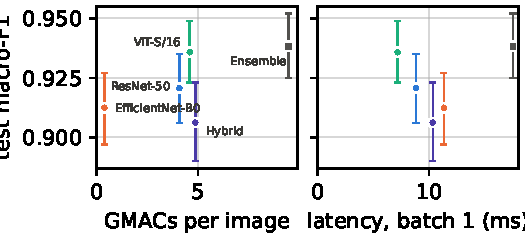
\includegraphics[width=\columnwidth]{figures/cost.pdf}
\caption{Test macro-F1 (95\,\% CI) versus compute and single-image latency. Fewer MACs do not imply lower latency.}
\label{fig:cost}
\end{figure}

\begin{figure}[t]
\centering
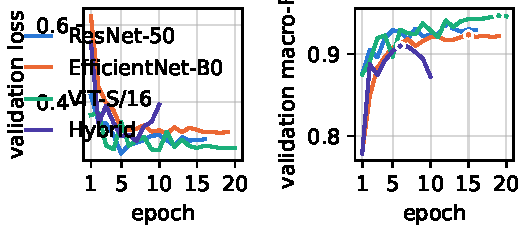
\includegraphics[width=\columnwidth]{figures/convergence.pdf}
\caption{Validation loss and macro-F1 per epoch; dots mark the epoch whose weights were kept.}
\label{fig:convergence}
\end{figure}

\subsection{Per-class performance and errors}
Pylorus, cecum and ulcerative colitis are nearly solved (Table~\ref{tab:perclass}). Esophagitis and normal Z-line are the
only classes below 0.90 F1 for every model, and their mutual confusion is the most frequent error (121 esophagitis
images predicted as Z-line and 83 Z-line images predicted as esophagitis, summed over the four models). ViT-S/16 is the
best on this pair (esophagitis recall 0.88), EfficientNet-B0 the worst (0.77). The hybrid has the best Z-line recall
(0.92) at the cost of the worst esophagitis recall (0.73), and its errors overlap the least with those of ViT-S/16
(Jaccard index 0.33, the lowest of all pairs), which explains its selection for the ensemble. The second confusion,
dyed resection margins versus dyed-lifted polyps, depends on whether the polyp has already been removed.

\begin{table}[t]
\caption{Test F1 per class}
\label{tab:perclass}
\centering
\footnotesize
\setlength{\tabcolsep}{2.6pt}
\begin{tabular}{@{}lcccccccc@{}}
\toprule
Model & D-pol & D-mar & Esoph & Cecum & Pylor & Z-line & Polyp & Colit \\
\midrule
Ensemble & 0.94 & 0.94 & \best{0.87} & 0.98 & 0.99 & \best{0.86} & 0.95 & 0.97 \\
ViT-S/16 & 0.94 & 0.94 & 0.86 & 0.98 & 0.99 & 0.85 & 0.96 & 0.97 \\
ResNet-50 & 0.93 & 0.94 & 0.84 & 0.97 & 0.98 & 0.84 & 0.92 & 0.95 \\
EffNet-B0 & 0.93 & 0.94 & 0.79 & 0.97 & 0.99 & 0.80 & 0.93 & 0.94 \\
Hybrid & 0.91 & 0.92 & 0.81 & 0.94 & 0.99 & 0.84 & 0.91 & 0.94 \\
\bottomrule
\end{tabular}
\end{table}

\subsection{Hyperparameter sensitivity}
Table~\ref{tab:sens} and Fig.~\ref{fig:sens} show the one-factor-at-a-time study. Pretraining is by far the largest
effect: EfficientNet-B0 and ViT-S/16 lose 0.259 and 0.187 macro-F1 when trained from scratch. A learning rate of
$10^{-5}$ leaves the model under-fitted after 20 epochs, and 64\,px inputs cost 0.053, confirming that fine detail
matters. Two predictions failed: $10^{-3}$ \emph{improved} EfficientNet-B0 (+0.015), so the shared learning rate was
conservative for it, and removing augmentation had no measurable effect within 20 epochs.

\begin{table}[t]
\caption{Sensitivity study: change in test macro-F1 relative to the pretrained baseline (EfficientNet-B0: 0.912;
ViT-S/16: 0.936), with paired bootstrap 95\,\% CIs}
\label{tab:sens}
\centering
\footnotesize
\setlength{\tabcolsep}{3pt}
\begin{tabular}{@{}llcc@{}}
\toprule
Run & Change & Macro-F1 & $\Delta$ [95\,\% CI] \\
\midrule
B0 & LR $10^{-4}\rightarrow10^{-5}$ & 0.806 & $-$0.107 [$-$0.129, $-$0.086] \\
B0 & LR $10^{-4}\rightarrow10^{-3}$ & 0.927 & +0.015 [+0.002, +0.030] \\
B0 & batch 32$\rightarrow$128 & 0.898 & $-$0.014 [$-$0.029, $-$0.002] \\
B0 & 224$\rightarrow$64\,px & 0.859 & $-$0.053 [$-$0.074, $-$0.034] \\
B0 & no augmentation & 0.913 & +0.001 [$-$0.013, +0.013] \\
B0 & from scratch & 0.654 & $-$0.259 [$-$0.287, $-$0.233] \\
ViT-S & from scratch & 0.749 & $-$0.187 [$-$0.211, $-$0.162] \\
\bottomrule
\end{tabular}
\end{table}

\begin{figure}[t]
\centering
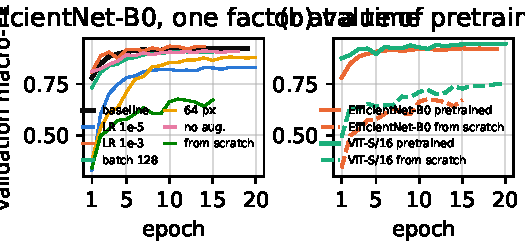
\includegraphics[width=\columnwidth]{figures/sensitivity.pdf}
\caption{Validation macro-F1 of the sensitivity runs. Dashed: training from scratch.}
\label{fig:sens}
\end{figure}

\subsection{Interpretability}
Fig.~\ref{fig:interp} shows the explanation maps. ResNet-50 produces the sharpest Grad-CAM maps, centered on the dye,
the pyloric opening or the inflamed junction; EfficientNet-B0's maps are broader. The ViT-S/16 rollout is diffuse and
spreads over the image, and in the dyed-margin example it highlights the ScopeGuide box. The hybrid's rollout is the
most focused, often on a few lesion patches. On the esophagitis$\rightarrow$Z-line failures (Fig.~\ref{fig:fail}) every
model looks at the gastro-esophageal junction: the errors come from the subtle visual difference, not from looking at
the wrong place.

\begin{figure*}[t]
\centering
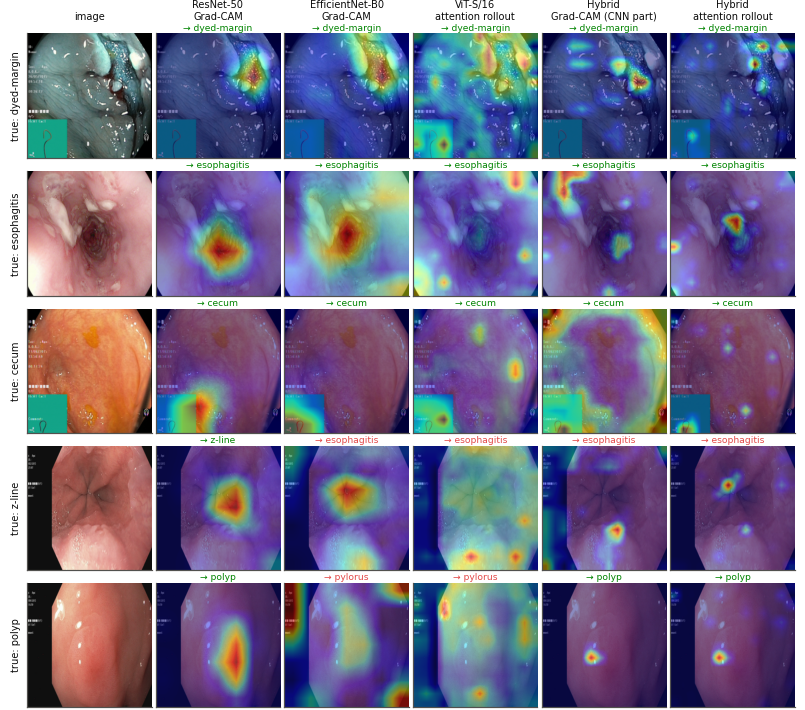
\includegraphics[width=0.86\textwidth]{figures/interpretability.png}
\caption{Grad-CAM (CNNs, hybrid's CNN part) and attention rollout (ViT-S/16, hybrid's Transformer layers) on test
images of five classes; the label above each map is the prediction (green: correct, red: wrong).}
\label{fig:interp}
\end{figure*}

\begin{figure*}[t]
\centering
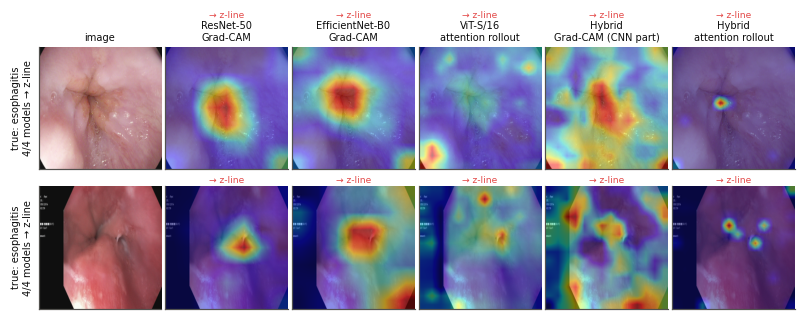
\includegraphics[width=0.86\textwidth]{figures/failure_cases.png}
\caption{Esophagitis images misclassified as normal Z-line by all four models: the maps are centered on the junction.}
\label{fig:fail}
\end{figure*}

\subsection{Shortcut learning}
\label{sec:shortcut}
The ScopeGuide display (a 3-D position indicator of the colonoscope) appears in 38\,\% of the images: in about 98\,\% of
cecum images, in a third to two thirds of the polyp, dyed and colitis images, and in none of the upper-GI classes
(Fig.~\ref{fig:scope}). Its presence thus reveals ``colonoscopy''. Masking it in the test images lowers the macro-F1 of
every model, with CIs that exclude zero (Table~\ref{tab:shortcut}). ResNet-50 is the most robust; the hybrid, whose
Transformer part attends to the box (rollout ratio 1.89) while its CNN part does not (0.79), is the most affected.
ViT-S/16 loses 0.025, slightly missing the success criterion of 0.02.

\begin{figure}[t]
\centering
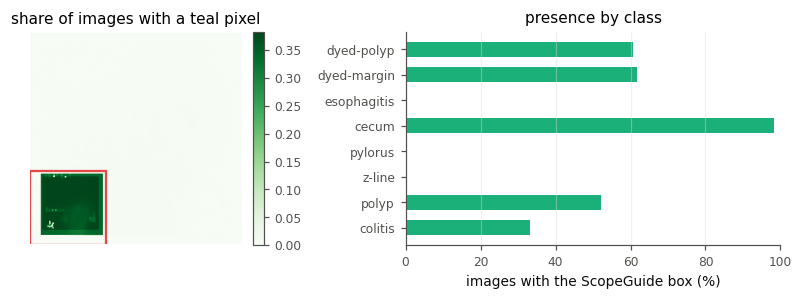
\includegraphics[width=\columnwidth]{figures/scopeguide.png}
\caption{Left: share of images with a teal pixel at each position (box region in red). Right: share of images of
each class containing the ScopeGuide box.}
\label{fig:scope}
\end{figure}

\begin{table}[t]
\caption{Shortcut test: macro-F1 change when the box is masked, share of changed predictions on the 452 test images
with the box, and explanation-map mass in the box relative to a uniform map}
\label{tab:shortcut}
\centering
\footnotesize
\setlength{\tabcolsep}{3pt}
\begin{tabular}{@{}lccc@{}}
\toprule
Model & $\Delta$ macro-F1 [95\,\% CI] & Changed (\%) & Map ratio \\
\midrule
ResNet-50 & \best{$-$0.014} [$-$0.024, $-$0.004] & \best{6.6} & \best{1.12} \\
EfficientNet-B0 & $-$0.028 [$-$0.042, $-$0.013] & 10.6 & 2.06 \\
ViT-S/16 & $-$0.025 [$-$0.038, $-$0.013] & 8.0 & 1.67 \\
Hybrid & $-$0.034 [$-$0.047, $-$0.021] & 12.6 & 0.79 / 1.89 \\
Ensemble & $-$0.026 [$-$0.038, $-$0.014] & 8.4 & -- \\
\bottomrule
\end{tabular}
\end{table}

\section{Discussion}
\textbf{Why ViT-S/16 won.} It combines global attention, tensor-core-friendly computation and, crucially, pretraining on
ImageNet-21k (14\,M images) against ImageNet-1k (1.3\,M) for the CNNs. Our design matched compute, not pretraining
data, so the result should be read as ``a well-pretrained Transformer'' rather than ``attention beats convolution'',
consistent with~\cite{matsoukas2021time}. It is also the best on the fine-grained esophagitis/Z-line pair and the
fastest per image, but its diffuse rollout maps are the hardest to explain to clinicians and it uses the box shortcut.

\textbf{Why the hybrid failed as a single model.} It discards the pretrained stage 4 of ResNet-50 and replaces it with
7.6\,M random weights; on 5{,}600 images the lost pretrained features outweigh the added global modelling, the same
lesson as the from-scratch runs. Its new layers, trained at a ten times larger learning rate, made validation loss rise
after epoch 7, and its attention learned the box shortcut. Yet its errors are the most complementary to ViT-S/16's,
which makes it a useful ensemble member.

\textbf{Why ResNet-50 and EfficientNet-B0 behave differently.} Both are statistically tied, but they suit different
purposes. ResNet-50 has the most localized explanations and the smallest shortcut dependence. EfficientNet-B0 has a
very low arithmetic cost but less capacity, which hurts on the hardest pair, and its latency advantage only appears in
batched inference. Its improvement at $10^{-3}$ shows that one shared learning rate slightly under-rates it.

\textbf{Which model for which use.} For the best single-model accuracy and for real-time GPU inference: ViT-S/16. For
low-power or edge hardware: EfficientNet-B0, which gives up 0.024 macro-F1 for twelve times fewer MACs. For explanations
shown to clinicians and robustness to the artifact: ResNet-50. The ensemble is only justified for offline second
reading, where its small gain is worth twice the compute.

\textbf{Limitations.} A single training seed (the CIs reflect test-set variability, not training variability);
unequal pretraining data between ViT and CNNs; one shared learning rate; a single dataset from one centre without
external validation; early stopping truncating the cosine schedule; a sensitivity study run one factor at a time on
one model, with the fine-tuning recipe for the from-scratch runs; and masking introduces a small distribution shift,
so the shortcut effect is an upper bound.

\section{Conclusion and Future Work}
On Kvasir v2, all four architectures exceed 0.90 macro-F1. A pretrained ViT-S/16 is the most accurate and fastest
single model, but the dominant factor is pretraining rather than architecture: training from scratch costs 0.19--0.26
macro-F1, six to nine times the spread between pretrained models, and a hybrid with half of its weights randomly
initialized underperforms its own CNN backbone. Efficiency depends on the deployment scenario, the remaining errors are
fine-grained (esophagitis versus Z-line), and every model partly exploits a colonoscopy-only display box. Future work
includes comparing CNNs pretrained on ImageNet-21k (e.g.\ BiT~\cite{kolesnikov2020bit}) to separate architecture from
pretraining, self-supervised pretraining on the unlabeled HyperKvasir frames, initializing the hybrid's Transformer
layers from pretrained weights, removing the ScopeGuide box during training with validation on other centres, higher
resolution and grade-level labels for esophagitis, and distilling the ensemble into a real-time model.

\section*{Reproducibility}
Code, the executed notebook and instructions are available at
\url{https://github.com/Yeldebao/AI-MASTERS/tree/main/deep-learning-kvasir}. The notebook downloads the dataset,
trains every model and regenerates all tables and figures in about 45 minutes on one NVIDIA L4 GPU (Google Colab).

\begin{thebibliography}{00}
\bibitem{pogorelov2017kvasir} K. Pogorelov \emph{et al.}, ``Kvasir: A multi-class image dataset for computer aided gastrointestinal disease detection,'' in \emph{Proc. 8th ACM Multimedia Systems Conf. (MMSys)}, 2017, pp. 164--169.
\bibitem{borgli2020hyperkvasir} H. Borgli \emph{et al.}, ``HyperKvasir, a comprehensive multi-class image and video dataset for gastrointestinal endoscopy,'' \emph{Scientific Data}, vol. 7, no. 283, 2020.
\bibitem{he2016resnet} K. He, X. Zhang, S. Ren, and J. Sun, ``Deep residual learning for image recognition,'' in \emph{Proc. IEEE CVPR}, 2016, pp. 770--778.
\bibitem{tan2019efficientnet} M. Tan and Q. V. Le, ``EfficientNet: Rethinking model scaling for convolutional neural networks,'' in \emph{Proc. ICML}, 2019, pp. 6105--6114.
\bibitem{dosovitskiy2021vit} A. Dosovitskiy \emph{et al.}, ``An image is worth 16x16 words: Transformers for image recognition at scale,'' in \emph{Proc. ICLR}, 2021.
\bibitem{chen2021transunet} J. Chen \emph{et al.}, ``TransUNet: Transformers make strong encoders for medical image segmentation,'' arXiv:2102.04306, 2021.
\bibitem{dai2021coatnet} Z. Dai, H. Liu, Q. V. Le, and M. Tan, ``CoAtNet: Marrying convolution and attention for all data sizes,'' in \emph{Proc. NeurIPS}, 2021.
\bibitem{steiner2022augreg} A. Steiner \emph{et al.}, ``How to train your ViT? Data, augmentation, and regularization in vision transformers,'' \emph{Trans. Mach. Learn. Res.}, 2022.
\bibitem{matsoukas2021time} C. Matsoukas, J. F. Haslum, M. S\"oderberg, and K. Smith, ``Is it time to replace CNNs with transformers for medical images?'' in \emph{ICCV Workshop on Computer Vision for Automated Medical Diagnosis}, 2021.
\bibitem{pogorelov2018medico} K. Pogorelov \emph{et al.}, ``Medico multimedia task at MediaEval 2018,'' in \emph{Proc. MediaEval Workshop}, 2018.
\bibitem{jha2020kvasirseg} D. Jha \emph{et al.}, ``Kvasir-SEG: A segmented polyp dataset,'' in \emph{Proc. Int. Conf. MultiMedia Modeling (MMM)}, 2020, pp. 451--462.
\bibitem{thambawita2020extensive} V. Thambawita \emph{et al.}, ``An extensive study on cross-dataset bias and evaluation metrics interpretation for machine learning applied to gastrointestinal tract abnormality classification,'' \emph{ACM Trans. Comput. Healthcare}, vol. 1, no. 3, 2020.
\bibitem{litjens2017survey} G. Litjens \emph{et al.}, ``A survey on deep learning in medical image analysis,'' \emph{Medical Image Analysis}, vol. 42, pp. 60--88, 2017.
\bibitem{raghu2019transfusion} M. Raghu, C. Zhang, J. Kleinberg, and S. Bengio, ``Transfusion: Understanding transfer learning for medical imaging,'' in \emph{Proc. NeurIPS}, 2019.
\bibitem{touvron2021deit} H. Touvron \emph{et al.}, ``Training data-efficient image transformers \& distillation through attention,'' in \emph{Proc. ICML}, 2021.
\bibitem{liu2021swin} Z. Liu \emph{et al.}, ``Swin Transformer: Hierarchical vision transformer using shifted windows,'' in \emph{Proc. IEEE/CVF ICCV}, 2021.
\bibitem{shamshad2023survey} F. Shamshad \emph{et al.}, ``Transformers in medical imaging: A survey,'' \emph{Medical Image Analysis}, vol. 88, 102802, 2023.
\bibitem{selvaraju2017gradcam} R. R. Selvaraju \emph{et al.}, ``Grad-CAM: Visual explanations from deep networks via gradient-based localization,'' in \emph{Proc. IEEE ICCV}, 2017, pp. 618--626.
\bibitem{abnar2020rollout} S. Abnar and W. Zuidema, ``Quantifying attention flow in transformers,'' in \emph{Proc. ACL}, 2020, pp. 4190--4197.
\bibitem{geirhos2020shortcut} R. Geirhos \emph{et al.}, ``Shortcut learning in deep neural networks,'' \emph{Nature Machine Intelligence}, vol. 2, pp. 665--673, 2020.
\bibitem{degrave2021covid} A. J. DeGrave, J. D. Janizek, and S.-I. Lee, ``AI for radiographic COVID-19 detection selects shortcuts over signal,'' \emph{Nature Machine Intelligence}, vol. 3, pp. 610--619, 2021.
\bibitem{loshchilov2019adamw} I. Loshchilov and F. Hutter, ``Decoupled weight decay regularization,'' in \emph{Proc. ICLR}, 2019.
\bibitem{loshchilov2017sgdr} I. Loshchilov and F. Hutter, ``SGDR: Stochastic gradient descent with warm restarts,'' in \emph{Proc. ICLR}, 2017.
\bibitem{goyal2017large} P. Goyal \emph{et al.}, ``Accurate, large minibatch SGD: Training ImageNet in 1 hour,'' arXiv:1706.02677, 2017.
\bibitem{szegedy2016rethinking} C. Szegedy, V. Vanhoucke, S. Ioffe, J. Shlens, and Z. Wojna, ``Rethinking the Inception architecture for computer vision,'' in \emph{Proc. IEEE CVPR}, 2016, pp. 2818--2826.
\bibitem{efron1993bootstrap} B. Efron and R. J. Tibshirani, \emph{An Introduction to the Bootstrap}. Chapman \& Hall, 1993.
\bibitem{mcnemar1947} Q. McNemar, ``Note on the sampling error of the difference between correlated proportions or percentages,'' \emph{Psychometrika}, vol. 12, no. 2, pp. 153--157, 1947.
\bibitem{dietterich1998tests} T. G. Dietterich, ``Approximate statistical tests for comparing supervised classification learning algorithms,'' \emph{Neural Computation}, vol. 10, no. 7, pp. 1895--1923, 1998.
\bibitem{kolesnikov2020bit} A. Kolesnikov \emph{et al.}, ``Big Transfer (BiT): General visual representation learning,'' in \emph{Proc. ECCV}, 2020.
\end{thebibliography}

\end{document}
